\chapter{Analyse verschiedener Fahrszenarien und Interpretation des Lösungsraumes}\label{cha:Ergebnisse}
In diesem Kapitel wird das im vorangegangenen Kapitel hergeleitete Gesamtsystem mit den Methoden aus Kapitel \ref{cha:Optimierung} für verschiedene Fahrszenarien gelöst. Dazu werden zunächst einige Vereinfachungen getroffen, mit denen es teilweise möglich ist, eine analytische Lösung zu finden. Die Erkenntnisse der einfacheren Szenarien werden dann verwendet, um die Lösungen komplexerer Szenarien zu interpretieren. 

\section{Geradeausfahrt}
Als erstes wird das Szenario einer reinen Geradeausfahrt betrachtet. Dazu wird das Fahrzeugmodell auf die Bewegung in longitudinaler Richtung reduziert und angenommen, dass sich das Fahrzeug exakt auf der Referenzkurve mit $\kapparefofs = 0$ bewegt - die querdynamischen Größen $d_r, \psi_r$ und $\kappa$ werden dabei vernachlässigt. Da sich das Fahrzeug auf der Referenzkurve befindet, ist durch $s_r$ die exakt vom Fahrzeug zurückgelegte Strecke gegeben. Die Systemdynamik des Fahrzeugs ist dann durch die Gleichungen 
\begin{align}
\dot{s}_r &= v \\
\dot{v} &= a_x \\
\dot{a}_x &= j_x \,,
\end{align}
vollständig beschrieben - es ergibt sich ein Integratorsystem 3. Ordnung. Die einzige Stellgröße ist in diesem Fall der Längsruck $j_x$.

\subsection{Lösungsraum bei energieoptimalem Gütefunktional}
Zunächst wird die Lösung des Szenarios Geradeausfahrt für ein energieoptimales Gütefunktional bestimmt. Wird im Gütefunktional die Stellgröße eines Systems bestraft, so wird von einem energieoptimalen Gütefunktional gesprochen, da das Ziel der Optimierung darin besteht, die benötigte Stellgröße möglichst gering zu halten. Diese ist häufig direkt mit der aufzuwendenden Energie verknüpft \cite{KnutGraichen.2012}. Wird zusätzlich noch die Endzeit als Gütekriterium bestraft, so ergibt sich in dem vereinfachten Szenario Geradeausfahrt das Gütefunktional
\begin{equation}
	J(\ve{x},\ve{u},t,t_f) = t_f + \int_{t_0}^{t_f}\frac{1}{2}f_uu^2\dtint{t} = t_f + \int_{t_0}^{t_f}\frac{1}{2}\fjx j_x^2\dtint{t}\,.
\end{equation}
Die Formulierung eines Integratorsystems mit einem energieoptimalen Gütefunktional soll nachfolgend verallgemeinert betrachtet werden. Wird die Stellgröße eines Integratorsystems mit der Ordnung $n$ als die $n$-te Ableitung des ersten Zustands gewählt, kann das Gütefunktional als 
\begin{equation}
J(\ve{x},\ve{u},t,t_f) = t_f + \int_{t_0}^{t_f}\frac{1}{2}f_u{x_1^{(n)}}^2\dtint{t}\,.
\end{equation}
geschrieben werden, wobei der eingeklammerte Hochindex $(n)$ die $n$-te Zeitableitung bezeichnet. Die Hamilton-Funktion ergibt sich zu
\begin{equation}
H(\ve{x},\ve{u},\ve{\lambda},t) = \frac{1}{2}f_u{x_1^{(n)}}^2 + \lambda_1x_1^{(1)} + \lambda_2x_1^{(2)} + ... + \lambda_nx_1^{(n)}
\end{equation}
und die adjungierten \gls{DGL} lauten dann  
\begin{align}
	\dot{\lambda_1} &= 0 \\
	\dot{\lambda_2} &= -\lambda_1 \\
	&\vdots \\
	\dot{\lambda_n} &= -\lambda_{n-1}\,.
\end{align}
Daraus wird ersichtlich, dass sich mit $x_1^{(n)} = -\frac{\lambda_n}{f_u}$ alle Zeitverläufe durch Integration ausgehend von $\lambda_1 = \textrm{konst.}$ bestimmen lassen. Dabei erhält man Polynome deren Grad mit jeder Integration um eins steigt. Bei einem System $n$-ter Ordnung müssen insgesamt $2n$ Integrationen durchgeführt werden, sodass die Lösung von $x_1$ ein Polynom vom Grad $2n-1$ darstellt. Der höchste Polynomgrad ist also immer ungerade. Dabei lässt sich feststellen, dass der Einfluss der höheren Exponenten der Polynome durch die mehrfache Integration abnimmt. Der Lösungsraum lässt sich wie folgt geschlossen angeben: 
\begin{align}
\begin{split}
\lambda_1 &= c_1 
\end{split}
\\
\begin{split}
\lambda_2 &= -c_1t + c_2 
\end{split}
\\
\begin{split}
&\vdots 
\end{split}
\\
\begin{split}
\lambda_n &= (-1)^{n-1}\frac{c_1}{(n-1)!}t^{n-1} + (-1)^{n-2}\frac{c_2}{(n-2)!}t^{n-2} + ... + (-1)^1c_{n-1}t + c_n 
\end{split}
\\
\begin{split}
x_n &= (-1)^n\frac{c_1}{f_u(n)!}t^{n} + (-1)^{n-1}\frac{c_2}{(n-1)!}t^{n-1} + ... - \frac{c_{n}}{f_u}t + x_{n,0} 
\end{split}
\\
\begin{split}
x_{n-1} &= (-1)^n\frac{c_1}{f_u(n+1)!}t^{n+1} + (-1)^{n-1}\frac{c_2}{(n)!}t^{n} + ... - \frac{c_{n}}{2f_u}t^2 + x_{n,0}t + x_{n-1,0} 
\end{split}
\\
\begin{split}
&\vdots 
\end{split}
\\
\begin{split}
x_{1} &= (-1)^n\frac{c_1}{f_u(2n-1)!}t^{2n-1} + (-1)^{n-1}\frac{c_2}{(2n-2)!}t^{2n-2} + ... - \frac{c_{n}}{f_u(n)!}t^n + ... \\
&\qquad ... + \frac{x_{n,0}}{(n-1)!}t^{n-1} + \frac{x_{n-1,0}}{(n-2)!}t^{n-2} + ... + x_{2,0}t + x_{1,0}
\end{split}
\end{align}
Damit lautet die Lösung des Integratorsystems 3. Ordnung für die Geradeausfahrt
\begin{align}
\begin{split}
\lambda_1 &= c_1 
\end{split}
\\
\begin{split}
\lambda_2 &= -c_1t + c_2 
\end{split}
\\
\begin{split}
\lambda_3 &= \frac{c_1}{2}t^2 - c_2t + c_3 
\end{split}
\\
\begin{split}
a_x &= -\frac{c_1}{6\fjx}t^3 + \frac{c_2}{2\fjx}t^2 - \frac{c_3}{\fjx}t + c_a
\end{split}
\\
\begin{split}
v &= -\frac{c_1}{24\fjx}t^4 + \frac{c_2}{6\fjx}t^3 - \frac{c_3}{2\fjx}t^2 + c_at + c_v
\end{split}
\\
\begin{split}
s &= -\frac{c_1}{120\fjx}t^5 + \frac{c_2}{24\fjx}t^4 - \frac{c_3}{6\fjx}t^3 + \frac{c_a}{2}t + c_vt + c_s
\end{split}
\end{align}
Letztendlich können die in den Gleichungen auftretenden unbekannten Integrationskonstanten $c_1, c_2, c_3,$ $c_a, c_v$ und $c_s$ mithilfe der Randbedingungen \eqref{eq:Anfangswerte}-\eqref{eq:Lambdaend} bestimmt und damit das Optimierungsproblem gelöst werden. Im Fall, dass der Endzeitpunkt frei ist, kann $t_f$ unter Zuhilfenahme von Gleichung \eqref{eq:Transversalitaet} bestimmt werden. Die dynamischen Gleichungen des Gesamtsystems können auch in der für die Beschreibung linearer Systeme üblichen Matrixschreibweise $\dz = \mat{A}\ve{z}$ geschrieben werden. Mit $\ve{z} = \begin{bmatrix}\ve{x}^T & \ve{\lambda}^T\end{bmatrix}^T$ lautet das lineare System \begin{equation}
	\dz = \begin{bmatrix}
	0 & 1 & 0 & 0 & 0 & 0 \\
	0 & 0 & 1 & 0 & 0 & 0 \\
	0 & 0 & 0 & 0 & 0 & -\frac{1}{\fjx} \\
	0 & 0 & 0 & 0 & 0 & 0 \\
	0 & 0 & 0 & -1 & 0 & 0 \\
	0 & 0 & 0 & 0 & -1 & 0 \\
	\end{bmatrix}\ve{z}\,,
\end{equation}
dessen Eigenwerte erwartungsgemäß alle in Null liegen und das reine Integrationsverhalten des Systems widerspiegeln.

\subsection{Lösungsraum bei Gütefunktional mit Bestrafung von Längsruck und -beschleunigung}
Wird nun neben dem energieoptimalen Anteil noch die ebenfalls komfortrelevante Größe Längsbeschleunigung berücksichtigt, lautet das Gütefunktional für die Geradeausfahrt 
\begin{equation}
J(\ve{x},\ve{u},t,t_f) = t_f + \int_{t_0}^{t_f}\frac{1}{2}\fjx j_x^2 + \frac{1}{2}\fax a_x^2\dtint{t}\,.
\end{equation}
Analog zum Vorgehen aus dem vorherigen Abschnitt können die adjungierten \gls{DGL} aufgestellt werden. Diese lauten nun
\begin{align}
\dot{\lambda_1} &= 0 \\
\dot{\lambda_2} &= -\lambda_1 \\
\dot{\lambda_3} &= -(\fax a_x + \lambda_2)\,. \label{eq:dlambda3_Geradeausfahrt}
\end{align}
Das lineare System lässt sich mit \begin{equation}
\dz = \begin{bmatrix}
0 & 1 & 0 & 0 & 0 & 0 \\
0 & 0 & 1 & 0 & 0 & 0 \\
0 & 0 & 0 & 0 & 0 & -\frac{1}{\fjx} \\
0 & 0 & 0 & 0 & 0 & 0 \\
0 & 0 & 0 & -1 & 0 & 0 \\
0 & 0 & -\fax & 0 & -1 & 0 \\
\end{bmatrix}\ve{z}
\end{equation}
angeben und besitzt im Gegensatz zu dem linearen System aus dem vorherigen Abschnitt zwei Eigenwerte bei $\pm\sqrt{\frac{\fax}{\fjx}}$. Die restlichen vier Eigenwerte liegen auch bei diesem System in Null. Es zeigt sich allerdings, dass neben dem integrierenden Verhalten auch stabile und instabile Eigenmoden auftreten. Auch in diesem Fall lässt sich die Lösung der \gls{DGL} analytisch berechnen. Die Lösung von $\lambda_2$ kann durch Integration der Konstanten $c_1$ bestimmt werden. Wird die Steuerungsgleichung $j_x = -\frac{\lambda_3}{\fjx}$ abgeleitet und in Gleichung \eqref{eq:dlambda3_Geradeausfahrt} eingesetzt, ergibt sich für die Beschleunigung eine gewöhnliche \gls{DGL} 2. Ordnung. Durch das Einsetzen erhält man die \gls{DGL}
\begin{equation}
\dot{j}_x = \ddot{a}_x = \frac{\fax}{\fjx}a_x + \frac{\lambda_2}{\fjx} = \frac{\fax}{\fjx}a_x - \frac{c_1}{\fjx}t + \frac{c_2}{\fjx} \,, \label{eq:DGL_ax}
\end{equation}
deren Lösung
\begin{equation}
a_x = k_1e^{\sqrt{\frac{\fax}{\fjx}}t} + k_2e^{-\sqrt{\frac{\fax}{\fjx}}t} + \frac{c_1}{\fax}t - \frac{c_2}{\fax} \, \label{eq:DGL_ax_Lösung}
\end{equation}
lautet, wobei die Faktoren $k_1$ und $k_2$ Konstanten bezeichnen, die bei der Lösung der \gls{DGL} entstehen. Durch zeitliches Differenzieren bzw. Integrieren können aus $a_x$ die Lösungen für $j_x, v$ und $s_r$ ermittelt werden. Diese lauten
\begin{align}
\begin{split}
j_x &= k_1\sqrt{\frac{\fax}{\fjx}}e^{\sqrt{\frac{\fax}{\fjx}}t} - k_2\sqrt{\frac{\fax}{\fjx}}e^{-\sqrt{\frac{\fax}{\fjx}}t} + \frac{c_1}{\fax} \label{eq:DGL_jx_Lösung}
\end{split}
\\
\begin{split}
v &= k_1\sqrt{\frac{\fjx}{\fax}}e^{\sqrt{\frac{\fax}{\fjx}}t} - k_2\sqrt{\frac{\fjx}{\fax}}e^{-\sqrt{\frac{\fax}{\fjx}}t} + \frac{c_1}{2\fax}t^2 - \frac{c_2}{\fax}t + c_v
\end{split}
\\
\begin{split}
s &= k_1\frac{\fjx}{\fax}e^{\sqrt{\frac{\fax}{\fjx}}t} + k_2\frac{\fjx}{\fax}e^{-\sqrt{\frac{\fax}{\fjx}}t} + \frac{c_1}{6\fax}t^3 - \frac{c_2}{2\fax}t^2 + c_vt + c_s \,.
\end{split}
\end{align}
Auch hier bestehen die Lösungen der Trajektorien zum Teil aus Polynomen. Allerdings sind die Polynomgrade um zwei geringer als bei der reinen energieoptimalen Lösung. Des Weiteren zeigt sich mit den Exponentialtermen der Einfluss der stabilen und instabilen Moden auf die Systemzustände. Es kann festgestellt werden, dass die optimalen Trajektorien mit geringerer Bestrafung der Längsbeschleunigung zunehmend gegen die Lösung der rein ruckoptimalen Lösung laufen, wie in Abbildung \ref{fig:var_fax} zu erkennen ist. Offenbar ergeben sich die Koeffizienten $k_1$ und $k_2$ der Exponentialanteile bei der Lösung des nichtlinearen Gleichungssystems derart, dass der Einfluss der ``fehlenden'' Polynomgrade durch die Exponentialfunktionen ersetzt wird. Die Abbildung macht außerdem deutlich, dass bereits eine Bestrafung der Längsbeschleunigung von $\fax = 0.05$, die um den Faktor 20 geringer ist, als die Bestrafung des Längsrucks, zu wesentlich niedrigeren Beschleunigungsverläufen und damit einem höheren Maß an Fahrkomfort führt. Dies geschieht auf Kosten der Reisezeit, da diese entsprechend ansteigt. 
\begin{figure}[h] 
	\centering
	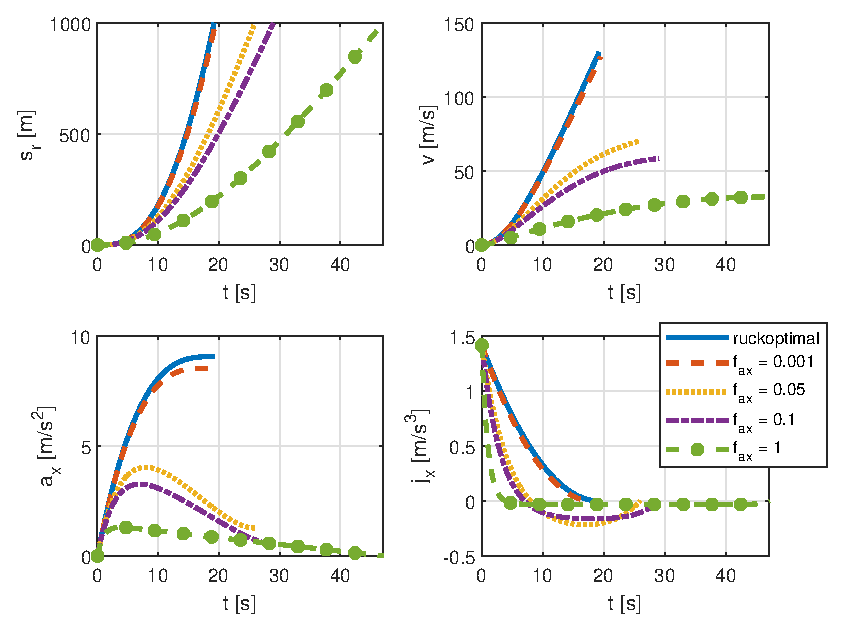
\includegraphics[width=0.8\linewidth]{./Bilder/Ergebnisse/Geradeausfahrt/var_fax.eps}
	\caption{Lösungstrajektorien der Fahrzeugzustände und der Stellgröße bei einer langen Geradeausfahrt mit $s_f=\valunit{1000}{m}$ und freien Endzuständen und freier Endzeit. Für abnehmende Bestrafung der Längsbeschleunigung nimmt die optimale Lösung immer mehr die Form der rein ruckoptimalen Lösung an. Der Ruck ist dabei mit $\fjx = 1$ gewichtet.}
	\label{fig:var_fax}
\end{figure}

\subsection{Lange Geradeausfahrt}
Ein Szenario, in dem die bisherigen Ergebnisse Anwendung finden ist die lange Geradeausfahrt, die nachfolgend eingehend analysiert werden soll. Zunächst wird die Lösung für $\fax = \fjx = 1$, also für gleiche Bestrafung von Beschleunigung und Ruck betrachtet. Das Szenario einer langen Geradeausfahrt zeichnet sich dadurch aus, dass sich der Zeitverlauf in drei Abschnitte unterteilen lässt. Im ersten Bereich für kleine Zeitpunkte gilt $0\leq t\ll t_f$, während im dritten Bereich nahe des Endzeitpunkts $0\ll t\leq t_f$ gilt. In dem Bereich dazwischen gilt $0\ll t\ll t_f$. Es zeigt sich, dass der Koeffizient des instabilen Teils $k_1$ sehr geringe Werte im Bereich von $10^{-40}\leq k_1 \leq 10^{-10}$ annimmt, wobei $k_2$ um einige Größenordnungen größer ist. Dies hat zur Folge, dass der Einfluss des instabilen Anteils erst für große $t$ (im dritten Zeitabschnitt) sichtbar wird und die Trajektorien divergieren, während das Verhalten für kleine $t$ (im ersten Zeitabschnitt) vom stabilen Teil dominiert wird und anschließend abklingt. Im Bereich dazwischen ist der Einfluss des stabilen Anteils bereits abgeklungen und der instabile Anteil ist noch nicht aufgeklungen. Folglich lässt sich die Aussage treffen, dass die Trajektorien für $t\ll t_f$ von links und für $0\ll t$ von rechts gegen den Polynomanteil konvergieren. Unter der Voraussetzung, dass die beiden Exponentialanteile jeweils nur in einem der drei Bereiche gelten, lassen sich die folgenden Annahmen treffen. Für den ersten Bereich kann der Einfluss der instabilen Mode mit $k_1(\cdot)e^{\sqrt{\frac{\fax}{\fjx}}t} \approx 0$ angenommen werden. Analog dazu gilt für den Einfluss des stabilen Anteils im dritten Bereich $k_2(\cdot)e^{-\sqrt{\frac{\fax}{\fjx}}t} \approx 0$. In diesen Bereichen gilt 
\begin{align}
j_x &\approx -k_2\sqrt{\frac{\fax}{\fjx}}e^{-\sqrt{\frac{\fax}{\fjx}}t} + \frac{c_1}{\fax} \quad\textrm{für}\quad 0\leq t\ll t_f \label{eq:j_Bereich_1} \\
a_x &\approx k_2e^{-\sqrt{\frac{\fax}{\fjx}}t} + \frac{c_1}{\fax}t - \frac{c_2}{\fax} \quad\textrm{für}\quad 0\leq t\ll t_f\,. \label{eq:a_Bereich_1}
\end{align}
sowie 
\begin{align}
j_x &\approx k_1\sqrt{\frac{\fax}{\fjx}}e^{\sqrt{\frac{\fax}{\fjx}}t} + \frac{c_1}{\fax} \quad\textrm{für}\quad 0\ll t\leq t_f \label{eq:j_Bereich_3} \\
a_x &\approx k_1e^{\sqrt{\frac{\fax}{\fjx}}t} + \frac{c_1}{\fax}t - \frac{c_2}{\fax} \quad\textrm{für}\quad 0\ll t\leq t_f\,. \label{eq:a_Bereich_3}
\end{align}
Die Trajektorien im zweiten Bereich lassen sich durch ihre Polynomanteile approximieren. Für die komfortrelevanten Größen Ruck und Beschleunigung gilt dann
\begin{align}
j_x &\approx \frac{c_1}{\fax} \quad\textrm{für}\quad 0\ll t\ll t_f \label{eq:j_Bereich_2}
\\
a_x &\approx \frac{c_1}{\fax}t - \frac{c_2}{\fax} \quad\textrm{für}\quad 0\ll t\ll t_f\,. \label{eq:a_Bereich_2}
\end{align}
Da die Trajektorien des Rucks und der Beschleunigung für lange Geradeausfahrten offenbar als Konstante bzw. Gerade betrachtet werden können, zu denen die Lösung sowohl von links als auch von rechts hin konvergiert, stellt sich die Frage, ob anhand der Kenntnis über den Lösungsraum, Beschränkungen für die Längsbeschleunigung angegeben werden können. 

\subsubsection{Begrenzung der Längsbeschleunigung}
Nachfolgend werden zwei Sets von Randbedingungen untersucht. Kenntnis über die Anfangszustände und damit Vorgabe der Anfangsbedingungen \xzero\,wird bei allen Szenarien vorausgesetzt. Allerdings kann die Vorgabe der Endwerte variiert werden. Zwei Sets an Endbedingungen erweisen sich bei der hier betrachteten langen Geradeausfahrt als besonders geeignet. Neben der Vorgabe einer Strecke $s_f$, die zurückgelegt werden soll und damit der Vorgabe des Endzustands für $s_r(t_f)$, können die Endgeschwindigkeit und -beschleunigung entweder festgelegt oder frei sein. Die Vorgabe von Endgeschwindigkeit und -beschleunigung ist sinnvoll, wenn das Fahrzeug unter Berücksichtigung des Gütefunktionals beispielsweise nach einer festgelegten Strecke unbeschleunigt zum Stehen gebracht werden soll. Wenn hingegen diese beiden Endzustände nicht festgelegt sind, weil das Ziel nur darin besteht, die vorgegebene Strecke unter Berücksichtigung des Gütefunktionals abzufahren, dann können diese Endzustände frei bleiben, wobei sich nach Gleichung \eqref{eq:Lambdaend} Endbedingungen für die adjungierten Zustände ergeben. 

\textbf{Feste Endgeschwindigkeit und feste Endbeschleunigung}

Zur Klärung der Frage, ob die Längsbeschleunigung beschränkt ist, kann eine Fallunterscheidung für die Vorzeichen der Koeffizienten $k_1$ und $k_2$ vorgenommen werden. So lässt sich feststellen, dass der stabile und instabile Anteil in Gleichung \eqref{eq:DGL_ax_Lösung} bei identischem Vorzeichen die gleiche Krümmungsrichtung haben (unabhängig davon, ob das Vorzeichen positiv oder negativ ist). Das bedeutet, dass die Exponentialanteile entweder beide von oben oder beide von unten gegen den linearen Lösungsanteil konvergieren. Für die Lösung des Rucks bedeuten identische Vorzeichen, dass die Krümmungen der Exponentialanteile in der Lösung in Gleichung \eqref{eq:DGL_jx_Lösung} immer entgegengesetzte Richtungen haben und einer der Anteile von oben gegen die Konstante konvergiert, während der andere Teil von unten gegen die Konstante läuft. Aufgrund des streng monotonen Verhaltens der Exponentialfunktionen, ist auch der Ruck über das gesamte Lösungsintervall streng monoton, sodass $j_x$ genau eine Nullstelle hat\footnote{Streng genommen muss diese Nullstelle nicht zwangsläufig innerhalb des Lösungsintervalls liegen.}. Dadurch, dass der Ruck genau eine Nullstelle besitzt, hat $a_x$ genau ein Extremum. Mit der Kenntnis, dass die Beschleunigung ausgehend vom Anfangswert $a_0$ gegen die Gerade in Bereich zwei konvergiert und anschließend unter Beibehaltung der Krümmungrichtung von der Geraden weg gegen den Endwert $a_f$ läuft, lasst sich feststellen, dass die Beschleunigung bei gleichem Vorzeichen der Koeffizienten $k_1$ und $k_2$ stets durch den linearen Anteil der Lösung und die Verbindungsgerade zwischen $a_0$ und $a_f$ beschränkt ist. In Abbildung \ref{fig:vf_af_fest_gleiches_VZ} sind die optimalen Lösungstrajektorien der Fahrzeugzustände $s_r$, $v$ und $a_x$ sowie der Stellgröße $j_x$ bei vorgegebenen Endzuständen und ansonsten identischer Parametrierung dargestellt. Die Anfangsgeschwindigkeit wurde so gewählt, dass die Vorzeichen der Lösungen von $k_1$ und $k_2$ identisch sind. Die Endzustände wurden so gewählt, dass das Fahrzeug nach \valunit{1000}{m} unbeschleunigt zum Stehen kommt. Der Endzeitpunkt wurde im Sinne einer einheitlichen Darstellung fest zu $t_f = \valunit{40}{s}$ gewählt. Das zuvor beschriebene Verhalten der Beschleunigungs- und Rucktrajektorien ist gut in den unteren beiden Graphen zu erkennen. Zum einen lassen sich die beiden Bereiche erkennen, in denen die Lösungen von den Exponentialteilen dominiert werden, sowie der mittlere Bereiche, in dem die Lösungen der Geraden für die Beschleunigung und der Konstanten für den Ruck entsprechen. Zudem zeigt die Abbildung unten links die Beschränkung der Beschleunigung (grau schattiert) durch die Verbindungsgerade der Randwerte und den linearen Anteil der Lösung.
\begin{figure}[h] 
	\centering
	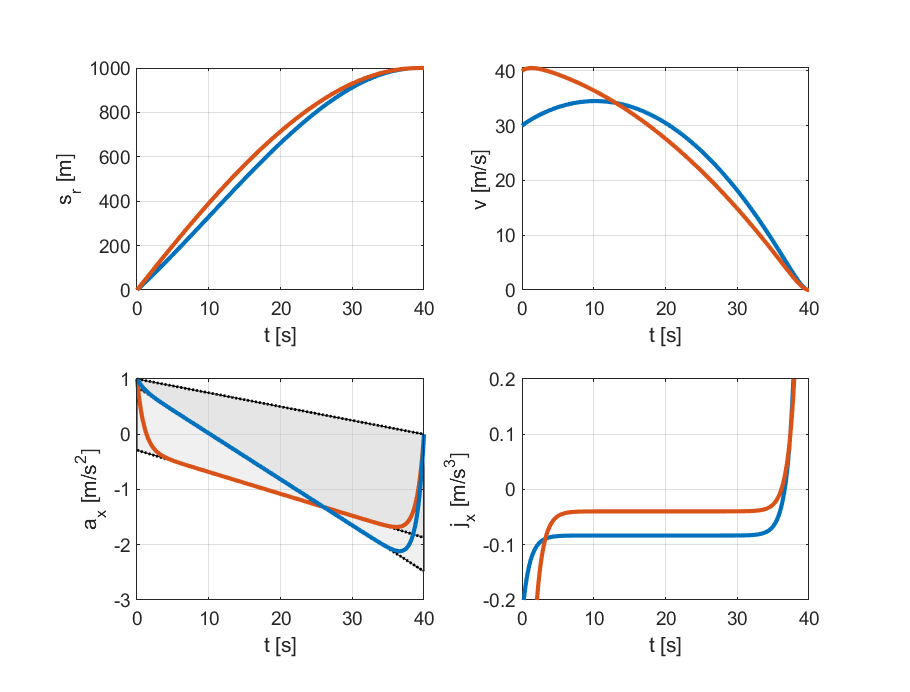
\includegraphics[width=\linewidth]{./Bilder/Ergebnisse/Geradeausfahrt/vf_af_fest_gleiches_VZ.eps}
	\caption{Lösungstrajektorien der Fahrzeugzustände und der Stellgröße bei einer langen Geradeausfahrt mit $s_f=\valunit{1000}{m}$ und fester Endgeschwindigkeit und -beschleunigung. Das Vorzeichen von $k_1$ und $k_2$ ist identisch.}
	\label{fig:vf_af_fest_gleiches_VZ}
\end{figure}

Für den Fall, dass das Vorzeichen der Koeffizenten $k_1$ und $k_2$ unterschiedlich ist, haben die Exponentialanteile in $j_x$ dieselbe Krümmungsrichtung und laufen damit beide entweder von oben oder von unten gegen die Konstante, während die Anteile in $a_x$ mit unterschiedlichen Vorzeichen wirken. Damit lässt sich feststellen, dass $j_x$ immer zwei Nullstellen besitzt, weshalb in $a_x$ zwei Extrema auftreten können. Da $j_x$ bei zwei Nullstellen einen Vorzeichenwechsel aufweist, hat die Steigung der Beschleunigung einen Richtungswechsel, woraus abgeleitet werden kann, dass es bei zwei Extrema ein Maximum und ein Minimum gibt und die Lösung von $a_x$ die Verbindungsgerade der Randwerte in einem Punkt schneidet. Dadurch, dass die Exponentialanteile der Lösung auch hier wieder gegen den linearen Anteil konvergieren, kann schließlich auch in diesem Fall argumentiert werden, dass die Beschleunigung stets durch die Verbindungsgerade von $a_0$ und $a_f$ und den linearen Anteil beschränkt ist, wobei sich die Geraden im mittleren Abschnitt bei 
\begin{equation}
t = \frac{a_0\fax + c_2}{c_1 - \frac{\fax(a_f - a_0)}{t_f}}
\end{equation} 
schneiden. Das Verhalten für diesen Lösungsfall ist in Abbildung \ref{fig:vf_af_fest_unterschiedliches_VZ} dargestellt. In den Graphen der Beschleunigung und des Rucks zeigt sich deutlich das beschriebene Verhalten mit den unterschiedlich gekrümmten Exponentialanteilen sowie die Konvergenz von links und rechts hin zu der jeweiligen Lösung auf dem mittleren Abschnitt. Außerdem ist die Beschränkung der Beschleunigung gut zu erkennen. 
\begin{figure}[h] 
	\centering
	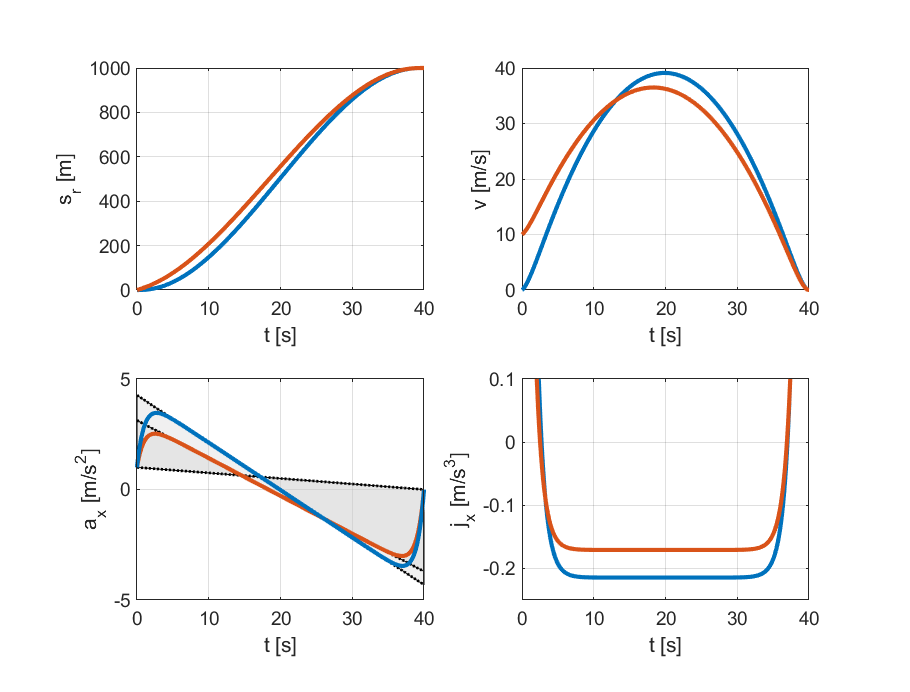
\includegraphics[width=\linewidth]{./Bilder/Ergebnisse/Geradeausfahrt/vf_af_fest_unterschiedliches_VZ.eps}
	\caption{Lösungstrajektorien der Fahrzeugzustände und der Stellgröße bei einer langen Geradeausfahrt mit $s_f=\valunit{1000}{m}$ und fester Endgeschwindigkeit und -beschleunigung. Das Vorzeichen von $k_1$ und $k_2$ ist unterschiedlich.}
	\label{fig:vf_af_fest_unterschiedliches_VZ}
\end{figure}

\textbf{Freie Endgeschwindigkeit und freie Endbeschleunigung}

Dadurch, dass die Endzustände $v(t_f)$ und $a_x(t_f)$ nicht festgelegt sind, ergeben sich die Endbedingungen $\lambda_2(t_f) = 0$ und $\lambda_3(t_f) = 0 \rightarrow j_x(t_f) = 0$. Bei dieser Wahl der Endbedingungen ist die analytische Herleitung der maximalen und minimalen Beschleunigung möglich, welche nachfolgend betrachtet werden soll.. Da $j_x$ bis auf die beiden Exponentialanteile konstant ist, kann argumentiert werden, dass der Ruck maximal zwei Nullstellen aufweist, wobei diese nicht in Bereich zwei liegen können (in diesem Bereich ist $j_x$ näherungsweise konstant). Ein Kontinuum an Nullstellen in Bereich zwei ist aufgrund des monotonen Verhaltens der Exponentialfunktionen nicht möglich, weshalb der Ruck im ersten und im dritten Bereich auf Nullstellen untersucht wird. Im ersten Bereich folgt mit $j_x \stackrel{!}{=} 0$ aus Gleichung \eqref{eq:j_Bereich_1}
\begin{equation}
	t_{z,1} = -\sqrt{\frac{\fjx}{\fax}}\ln{\Big(\frac{c_1}{k_2}\sqrt{\frac{\fjx}{\fax^3}}\Big)}\,. \label{eq:t_z_1}
\end{equation}
Dadurch, dass die Endgeschwindigkeit frei ist, ergibt sich die Endbedingung 
\begin{equation}
	\lambda_2(t_f) = -c_1t_f + c_2 \stackrel{!}{=} 0\,.
\end{equation}
Mit der Anfangsbedingung für die Beschleunigung $a_x(0) = a_0$ folgt aus Gleichung \eqref{eq:a_Bereich_1}
\begin{equation}
k_2 = a_0 + \frac{c_2}{\fax} = a_0 + \frac{c_1t_f}{\fax}\,.
\end{equation}
Wird dieser Zusammenhang in Gleichung \eqref{eq:t_z_1} eingesetzt, erhält man mit 
\begin{equation}
t_{z,1} = -\sqrt{\frac{\fjx}{\fax}}\ln{\Big(\frac{c_1}{a_0+\frac{c_1t_f}{\fax}}\sqrt{\frac{\fjx}{\fax^3}}\Big)}
\end{equation}
den Zeitpunkt des Nulldurchgang von $j_x$ im ersten Bereich, wobei dieser vom Anfangswert der Beschleunigung, den Gewichtungsfaktoren der Komfortkriterien, dem Endzeitpunkt und der Lösung von $\lambda_1$ abhängt. Einsetzen von $t_{z,1}$ in Gleichung \eqref{eq:a_Bereich_1} liefert den Extremwert der Beschleunigung an dieser Stelle mit 
\begin{equation}
a_{x_{z,1}} = c_1\sqrt{\frac{\fjx}{\fax^3}} -c_1\sqrt{\frac{\fjx}{\fax^3}}\ln{\Big(\frac{c_1}{a_0+\frac{c_1t_f}{\fax}}\sqrt{\frac{\fjx}{\fax^3}}\Big)} - \frac{c_1t_f}{\fax}\,. 
\end{equation}
Die zweite Nullstelle von $j_x$ resultiert in dieser Wahl der Randbedingungen direkt aus $j_x(t_f) = 0$. Der Ruck hat folglich immer bei $t_{z,2} = t_f$ ein Extremum. Aus Gleichung \eqref{eq:j_Bereich_3} folgt 
\begin{equation}
k_1 = -\frac{c_1\sqrt{\frac{\fjx}{\fax^3}}}{e^{\sqrt{\frac{\fax}{\fjx}}t_f}}\,.
\end{equation}
Eingesetzt in Gleichung \eqref{eq:a_Bereich_3} lautet die Beschleunigung der zweiten Extremstelle
\begin{equation}
a_{x_{z,2}} = -c_1\sqrt{\frac{\fjx}{\fax^3}} + \frac{c_1}{\fax}t_f - \frac{c_1t_f}{\fax} = -c_1\sqrt{\frac{\fjx}{\fax^3}}\,. 
\end{equation}
Es lässt sich also festhalten, dass bei freien Endzuständen eine Extremstelle der Beschleunigung bei $t_f$ liegt und eine im ersten Abschnitt. Da der Endwert der Beschleunigung bei positiver Steigung immer unter dem linearen Lösungsanteil und bei negativer Steigung oberhalb der Geraden liegt, ist die Beschränkung durch den linearen Anteil der Lösung streng genommen nicht mehr gültig. Dennoch ist die Gerade als Näherungslösung für die Beschränkung geeignet wie Abbildung \ref{fig:vf_af_frei} zeigt. In der Abbildung sind die optimalen Zustands- und Stellgrößentrajektorien für unterschiedliche Anfangsgeschwindigkeiten gezeigt, sodass der Ruck und die Beschleunigung jeweils einmal von unten und von oben gegen die Approximation in Bereich zwei konvergieren. Der kleine Ausschhnitt in der Mitte der Abbildung gehört zum Graph der Beschleunigung unten links und zeigt den vergrößerten Abschnitt im Bereich von \valunit{36}{s} bis \valunit{40}{s}. Dabei wird deutlich, dass der Endwert der Beschleunigung jeweils außerhalb der durch die Verbindungsgerade und den linearen Anteil der Beschleunigungstrajektorie eingeschlossenen Fläche liegt und damit streng genommen außerhalb der Beschränkung. Da diese Verfehlung allerdings nur einen geringen Einfluss hat, lässt sich der lineare Anteil trotzdem zumindest als Näherungslösung für die Beschränkung verwenden. Zudem zeigt die Abbildung die beiden Nullstellen von $j_x$ und damit Extremstellen von $a_x$, von denen eine jeweils bei $t_f$ liegt.
\begin{figure}[h] 
	\centering
	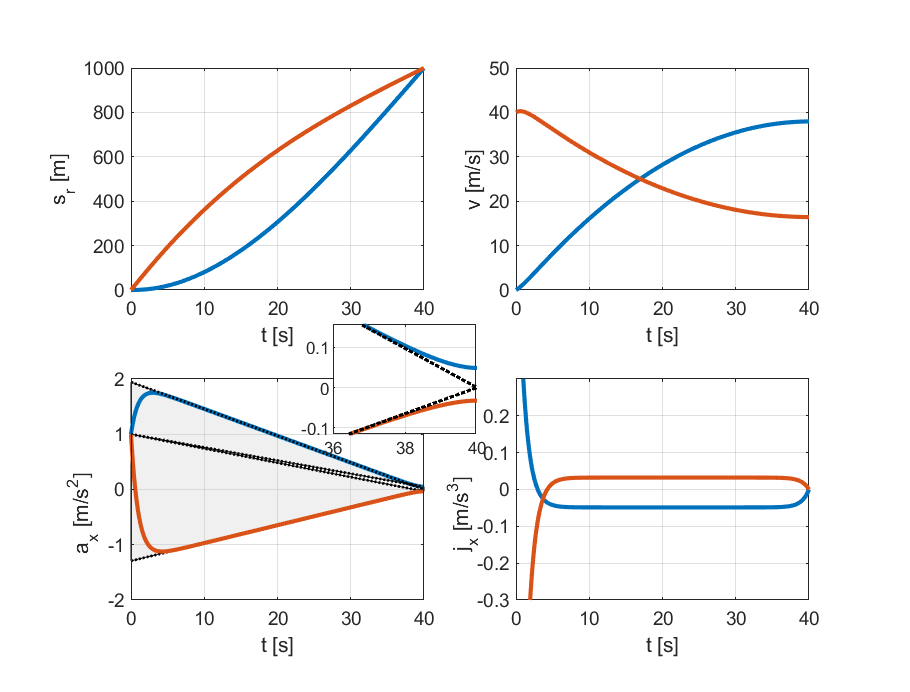
\includegraphics[width=\linewidth]{./Bilder/Ergebnisse/Geradeausfahrt/vf_af_frei_mit_zoom_aspectratio.eps}
	\caption{Lösungstrajektorien der Fahrzeugzustände und der Stellgröße bei einer langen Geradeausfahrt mit $s_f=\valunit{1000}{m}$ und freier Endgeschwindigkeit und -beschleunigung.}
	\label{fig:vf_af_frei}
\end{figure} 

Abschließend lässt sich festhalten, dass die analytischen Lösungen der optimalen Trajektorien für die Geradeausfahrt sowohl für ein rein energieoptimales Gütefunktional als auch für ein Gütefunktional mit zusätzlicher Bestrafung der Längsbeschleunigung bestimmt werden können und die verbleibenden Unbekannten mithilfe der Randbedingungen des Optimierungsproblems durch Lösung eines nichtlinearen Gleichungssystems berechnet werden können. Außerdem lässt sich unter Zuhilfenahme einiger Annahmen eine Abschätzung für die Beschränkung der Längsbeschleunigung treffen, über die wiederum Aussagen über den erwarteten Fahrkomfort getroffen werden können. Während der Anfangswert des Längsrucks nicht vorgegeben werden kann, sodass unter Umständen hohe Ruckwerte zu Beginn auftreten können, lässt sich der Endwert des Rucks bei freier Endbeschleunigung über die Endbedingung $\lambda_3(t_f) = 0$ vorgeben. 

\subsection{Heranfahren an eine Ampel bei bekannter Rotphase}\label{subsec:Ampelszenario}
Die Erkenntnisse über den Lösungsraum bei einer Geradeausfahrt mit beschleunigungs- und ruckoptimalem Gütefunktional werden nachfolgend verwendet, um das Heranfahren an eine Ampel mit bekannter Rotphase zu analysieren. Neben der Analyse des Anhalte- bzw. Anfahrvorgangs unter dem Aspekt des Fahrkomforts, dient dieses Szenario auch dem Vergleich zwischen vorausschauender Planung über die Ampelüberquerung hinaus und der weniger vorausschauenden zwei geteilten Planung bis zur Ampel und von dort aus bis zum Zielpunkt. Letzteres entspricht dabei dem vom Menschen gewählten Planungsverhalten, wobei die vorausschauende Variante einige Vorteile bietet. 

Das beschriebene Szenario kann als Geradeausfahrt interpretiert werden, bei der sich das Fahrzeug zu einem bestimmten Zeitpunkt $t_1$ an der Ampel befinden soll. Der Ort, an dem sich die Ampel befindet, kann dabei als die vom Startpunkt der Optimierung aus zurückzulegende Strecke $s_1$ betrachtet werden. Damit ein solches Szenario realistisch umsetzbar ist, muss die Strecke $s_1$ vom Fahrzeug bis zur Ampel, sowie der Zeitpunkt $t_1$ bekannt sein. Dieser wird als der Moment interpretiert, in dem die Ampel von rot auf grün springt und damit das Überqueren der Ampel für das Fahrzeug erlaubt ist\footnote{Ein Ansatz wie der Verkehrsfluss mithilfe von Fahrzeug zu Ampel Kommunikation und adaptiver Ampelphasen in Abhängigkeit des Verkehrsaufkommens verbessert werden kann, wurde in \cite{Gradinescu} untersucht.}. Das Szenario lässt sich dann mithilfe der internen \gls{GNB} $s_r(t_1) = s_1$ bei festem und bekanntem $t_1$ beschreiben. Alternativ kann das Szenario als zwei zusammengesetzte Geradenabschnitte verstanden werden, die an dem über die Zeit und die Strecke definierten Punkt $\mathcal{P}_1 = (t_1, s_1)$ miteinander verknüpft sind. Die Systemdynamik bleibt in den beiden Zeitabschnitten unverändert. Wird die insgesamt benötigte Zeit $t_f$ als Komfortkriterium verwendet, um möglichst schnell zum Zielort zu gelangen, dann kann das Szenario als ein Gesamtoptimierungsproblem mit der internen \gls{GNB} betrachtet werden, wobei $t_f$ über das gesamte Szenario bei der Optimierung berücksichtigt wird. Stattdessen kann das Szenario auch als zwei seperate Optimierungsprobleme formuliert werden, wobei das zweite Optimierungsproblem auf dem ersten aufsetzt, während bei den beiden Problemformulierungen nur das Verhalten im jeweiligen Zeitabschnitt $t_0 \leq t \leq t_1$ bzw. $t_1 \leq t \leq t_f$ berücksichtigt wird. Es sei an dieser Stelle darauf hingewiesen, dass die beiden Herangehensweisen das Problem zu formulieren nicht äquivalent sind und nicht zu erwarten ist, dass sie identische Ergebnisse liefern. Sie dienen aber der Unterscheidung zwischen dem erwarteten menschlichen Verhalten und dem maschinellen Verhalten eines automatisierten Fahrzeugs, was durch eine einfache Optimierung mit Blick auf das Gesamtintervall erreicht werden kann.

\subsubsection{Vorausschauende Planung}\label{subsubsec:Vorausschauend}
Zunächst soll die vorausschauende Planung des Heranfahrens an die Ampel untersucht werden. Das Optimierungsproblem für dieses Szenario kann wie folgt formuliert werden
\begin{align}
\min_{\ve{u}} \quad & J(\ve{x},\ve{u},t,t_f) = t_f + \int_{t_0}^{t_f}\frac{1}{2}\fjx j_x^2 + \frac{1}{2}\fax a_x^2\dtint{t} \\
\textrm{u.B.v.} \quad& \xoftzero = \xzero \\
& s_r(t_1) = s_1 \label{eq:srt1_gleich_s1}\\
& s_r(t_f ) = s_f\,,
\end{align}
wobei die Endzeit frei ist und als Optimierungsvariable betrachtet wird, während der Zeitpunkt $t_1$, zu dem die Ampel überquert werden soll, als fest betrachtet wird. Bis auf die festgelegte Zielstrecke $s_f$ sind die Endzustände frei. Das Ziel dieser Optimierung ist demnach, die Strecke $s_f$ möglichst schnell zurückzulegen unter Berücksichtigung der bekannten Ampelphase und des Fahrkomforts. Während die Beschreibung der Systemdynamik nicht verändert wird, stellt Gleichung \eqref{eq:srt1_gleich_s1} eine interne \gls{GNB} dar. Die Forderung nach Stetigkeit der Fahrzeugzustände im Übergangspunkt $\mathcal{P}_1$ führt zur Stetigkeitsbedingung 
\begin{equation}
\xoftoneminus = \xoftoneplus
\end{equation}
und schließlich zu der ersten Weierstrass-Erdmannschen-Eckenbedingung (siehe Kapitel \ref{sec:InterneGNB})
\begin{align}
2\tilde{\nu} - \lambda_1(t_1^-) + \lambda_1(t_1^+) &= 0\\
\lambda_2(t_1^-) + \lambda_2(t_1^+) &= 0\\
\lambda_3(t_1^-) + \lambda_3(t_1^+) &= 0\,. \label{eq:l3tminus_l3tplus}
\end{align}
Da $t_1$ fest ist, fällt die zweite Weierstrass-Erdmannschen-Eckenbedingung weg. Im Gegensatz zum menschlichen Planungsverhalten wird die vorausschauende Planung durch die Tatsache definiert, dass das Überqueren der Ampel am Punkt $\mathcal{P}_1$ über eine \gls{GNB} berücksichtigt wird, während die Gesamtzeit $t_f$ bei der Optimierung berücksichtigt wird.

\subsubsection{Menschliche Planung}\label{subsubsec:Mensch}
Bei der menschlichen Planung hingegen lässt sich das Optimierungsproblem, welches das selbe Gesamtziel hat - die Strecke $s_f$ unter Berücksichtigung der Ampelphase möglichst schnell zurückzulegen - in zwei Teilprobleme unterteilen. Für das Gesamtproblem gilt
\begin{equation}
\min_{\ve{u}} \, J(\ve{x},\ve{u},t,t_f) = \min_{\ve{u}} \, J_1(\ve{x},\ve{u},t,t_1) + \min_{\ve{u}} \, J_2(\ve{x},\ve{u},t,t_2)\,.
\end{equation}
Die Teilprobleme $J_1$ und $J_2$ lassen sich dabei wie folgt formulieren
\begin{multicols}{2}
	\begin{align}
	J_1(\ve{x},\ve{u},t,t_1) &= t_1 + \int_{t_0}^{t_1}\frac{1}{2}\fjx j_x^2 + \frac{1}{2}\fax a_x^2\dtint{t} \\
	\textrm{u.B.v.} \quad \xoftzero &= \xzero \\
	s_r(t_1) &= s_1 
	\end{align}
	\columnbreak
	\begin{align}
	J_2(\ve{x},\ve{u},t,t_f) &= (t_f - t_1) + \int_{t_1}^{t_f}\frac{1}{2}\fjx j_x^2 + \frac{1}{2}\fax a_x^2\dtint{t} \\
	\textrm{u.B.v.} \quad \xoftone &= \ve{x}_1 \\
	s_r(t_f) &= s_f 
	\end{align}
\end{multicols}
Diese lassen sich getrennt voneinander lösen und anschließend zur Lösung des Gesamtproblems zusammensetzen. Die Gesamtzeit wird in dieser Art der Problemformulierung also dadurch berücksichtigt, dass die Zeiten der beiden Teilprobleme optimiert werden, wobei das Fahrzeugverhalten für $t>t_1$ im ersten Teilproblem nicht berücksichtigt werden kann und umgekehrt. Der Anfangszustand $\ve{x}_1$ des zweiten Teilproblems entspricht der Lösung des ersten Teilproblems zum Zeitpunkt $t_1$.

\subsubsection{Vergleich der Planungsstrategien}\label{subsubsec:Vergleich}
In Abbildung \ref{fig:svaj_zoomj} sind die optimalen Trajektorien für die beiden erläuterten Planungsstrategien für zwei unterschiedliche Anfangsgeschwindigkeiten dargestellt. In den dargestellten Fällen wurde die Gewichtung $\fax = 1$ und $\fjx = 1$ gewählt. Außerdem wurden der Ort und die Zeit, zu denen die Ampel überquert werden soll, zu $\mathcal{P}_1 = (\valunit{40}{s}, \valunit{350}{m})$ gewählt. Die Gesamtstrecke beträgt $s_f = \valunit{600}{m}$. Wird zunächst nur das Verhalten der vorausschauenden Planung betrachtet (durchgezogene Linien), so fällt ein Unterschied im Beschleunigungsverhalten bzw. im Geschwindigkeitsprofil auf. Startet das Fahrzeug mit einer niedrigen Geschwindigkeit ($v_0 = \valunit{5}{\frac{\unit{m}}{\unit{s}}}$, blaue Linie), beginnt das Fahrzeug sofort zu beschleunigen und die Geschwindigkeit zu erhöhen und überquert die Ampel mit $v(t_1) = \valunit{16{,}78}{\frac{\unit{m}}{\unit{s}}}$. Für den Fall, dass das Fahrzeug bereits mit einer vergleichsweise hohen Geschwindigkeit startet ($v_0 = \valunit{15}{\frac{\unit{m}}{\unit{s}}}$, rote Linie), muss die Geschwindigkeit zunächst gedrosselt werden, damit die Ampel nicht zu früh überquert und damit die Rotphase der Ampel gerissen wird. Die Ampel wird in diesem Fall bei $\mathcal{P}_1$ mit $v(t_1) = \valunit{13{,}02}{\frac{\unit{m}}{\unit{s}}}$, also mit geringerer Geschwindigkeit, passiert. Beim Beschleunigungsverhalten zeigt sich, dass der Betrag der Trajektorie bei einer niedrigeren Startgeschwindigkeit geringere Werte annimmt und daher komfortabler ist im Vergleich zum Starten mit hoher Anfangsgeschwindigkeit. Die niedrigere Startgeschwindigkeit erreicht jedoch nicht nur aus Sicht der Beschleunigung ein höheres Maß an Fahrkomfort. Gleichzeitig lässt sich das Planungsziel schneller erreichen, da das anfängliche Abbremsen nicht notwendig ist und stattdessen von Beginn an gleichmäßig beschleunigt werden kann. In beiden Fällen lässt sich zudem aufgrund der Bedingung \eqref{eq:l3tminus_l3tplus} Stetigkeit für $j_x$ erreichen und so insgesamt ruckarme Lösungen erzielen. Betrachtet man nun die Lösungen bei der menschlichen Planung (gestrichelte Linien), lassen sich die selben qualitativen Zusammenhänge erkennen. Auch bei dieser Art der Planung ist es günstiger mit einer geringeren Geschwindigkeit zu starten, da sich das Ziel dadurch schneller erreichen lässt und geringere Beschleunigungen benötigt werden. Vor allem fällt jedoch auf, dass aufgrund der zweifachen Planungen, die bis auf den Anfangszustand unabhängig voneinander sind, in beiden Abschnitten der Anfangsruck nicht vorgegeben werden kann, sodass der Ruck unstetig ist und bei $\mathcal{P}_1$ eine Sprungstelle auftritt. Diese Sprungstelle führt zu deutlich größeren Ruckwerten als bei der vorausschauenden Planung. In \ref{Anhang} ist nochmals der Plot der Stellgröße dargestellt, allerdings mit einer weiteren Achsenskalierung, sodass die kompletten Ruckverläufe inklusive der Überhöhungen an der Sprungstelle zu erkennen sind. Neben den weniger komfortablen Rucktrajektorien, zeigt das Geschwindigkeitsprofil einen weiteren Nachteil der menschlichen Planung gegenüber der vorausschauenden Planung. Das menschliche Verhalten in der weniger vorausschauenden Planung wird damit begründet, dass die Planung abschnittsweise vom Startpunkt bis zur Ampel und von dort bis zum Zielpunkt stattfindet, ohne dass der Abschnitt nach der Ampel im ersten Abschnitt berücksichtigt wird. Dies hat zur Folge, dass die Geschwindigkeit $v(t_1)$ an der Ampel geringer ist, als sie im Idealfall bei vorausschauender Planung sein könnte, weshalb das Fahrzeug bei menschliche Planung immer mehr Zeit benötigt.
\begin{figure}[h] 
	\centering
	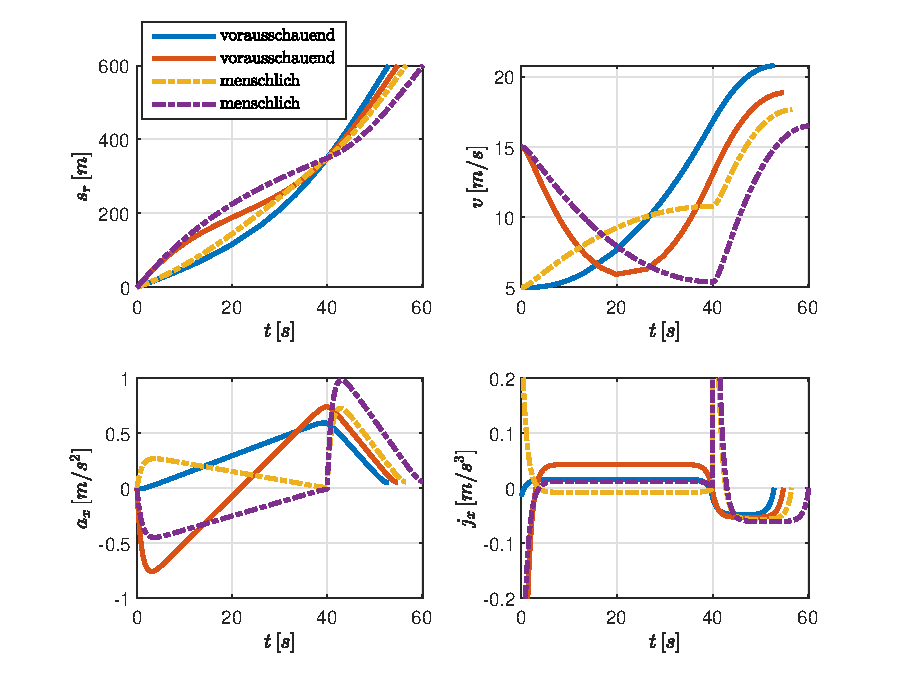
\includegraphics[width=\linewidth]{./Bilder/Ergebnisse/Geradeausfahrt/Ampel/v_5_v_15/svaj_zoomj.eps}
	\caption{Lösungstrajektorien der Fahrzeugzustände und der Stellgröße beim Zufahren auf eine Ampel mit bekannter Rotphase. Darstellung der Ergebnisse für vorausschauende und menschliche (weniger vorausschauend) Planung bei unterschiedlichen Startgeschwindigkeiten.}
	\label{fig:svaj_zoomj}
\end{figure} 

\textbf{Idealer Bremsvorgang}

Als Abschluss dieses Szenarios soll der Blick nochmal speziell auf den Bremsvorgang vor der Ampel bei hohen Anfangsgeschwindigkeiten gerichtet werden. Dazu sind in Abbildung \ref{fig:va_fa_variabel} die Geschwindigkeits- und Beschleunigungsverläufe von vorausschauender und menschlicher Planung für das Szenario mit der höheren Anfangsgeschwindigkeit gezeigt, allerdings mit unterschiedlichen Gewichtungen \fax\,der Beschleunigung. Dabei zeigt sich, dass die Geschwindigkeit an der Ampel am geringsten ist. Dieses Verhalten entspricht dabei am ehesten dem, wie sich eine fahrende Person im Straßenverkehr verhalten würde - man würde so lange die Geschwindigkeit reduzieren, bis die Ampel schließlich wieder auf grün springt. Bei der vorausschauenden Planung hingegen wird das Minimum deutlich früher erreicht. Dies mag auf den ersten Blick nicht gerade intuitiv erscheinen, da es bedeutet, dass schon stark verzögert wird, obwohl das Fahrzeug noch weit von der Ampel entfernt ist. Zudem bedeutet es, dass bereits beschleunigt wird, bevor die Ampel grün zeigt. Durch diese Weitsicht kann die Ampel allerdings mit höherer Geschwindigkeit überquert und das Endziel schneller erreicht werden. Die vorausschauende Planung mag zwar aus Sicht der Komfortkriterien besser abschneiden, als die menschliche Planung, allerdings ist sie nicht in allen Verkehrssituationen praktikabel. Bei besonders hohem Verkehrsaufkommen, bei dem sich der Verkehr möglicherweise vor einer Ampel staut, ist diese Art der Planung nicht sinnvoll nutzbar, da das Fahrzeug vor der Ampel keine freie Fahrt hat und dadurch nicht schon weit vor der Ampel beschleunigen kann, wie es von der Trajektorie verlangt wird. Zudem würde das starke Abbremsen weit vor der Ampel dazu führen, dass der nachfolgende Verkehr ausgebremst wird.
\begin{figure}[h] 
	\centering
	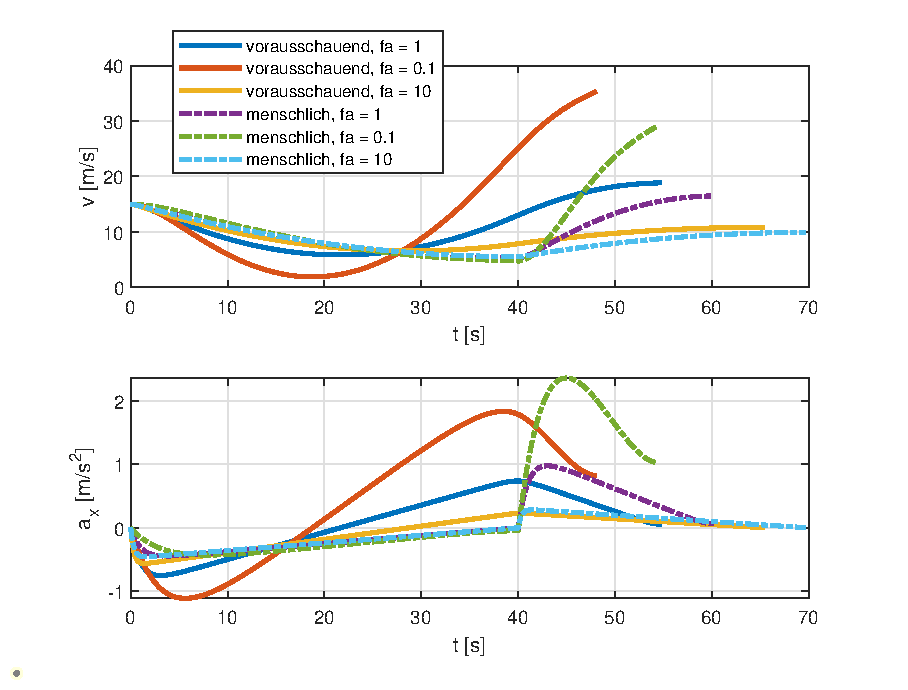
\includegraphics[width=0.9\linewidth]{./Bilder/Ergebnisse/Geradeausfahrt/Ampel/v_5_v_15/va_fa_variabel.eps}
	\caption{Geschwindigkeits- und Beschleunigungstrajektorien für vorausschauende und menschliche Planung für unterschiedliche Gewichtungen der Beschleunigung bei höherer Startgeschwindigkeit.}
	\label{fig:va_fa_variabel}
\end{figure} 
 

\section{Spurwechsel}\label{sec:Spurwechsel}
Bisher wurde ausschließlich die Längsdynamik des Fahrzeugs bei den untersuchten Szenarien berücksichtigt. Das nachfolgend untersuchte Szenario Spurwechsel stellt insofern eine Erweiterung der bisher betrachteten Szenarien dar, als dass nun unter Hinzunahme der querdynamischen Größen das Gesamtmodell des Fahrzeugs verwendet wird. Dadurch lassen sich Spurwechsel beschreiben und hinsichtlich der Querdynamik analysieren. 

\subsection{Komfortgewinn durch variable Gewichtung der Querabweichung}
\section{Kreisfahrt mit konstanter Krümmung}
Nachdem das Szenario Geradeausfahrt eingehend analysiert und diskutiert wurde, soll nachfolgend das Szenario einer Kreisfahrt untersucht werden. Die Kreisfahrt stellt mit seiner konstanten Krümmung einen vereinfachten Sonderfall einer Kurve dar. Durch die Analyse der Kreisfahrt lassen sich einige Erkenntnisse gewinnen, die später bei der Untersuchung allgemeiner Kurven mit veränderlicher Krümmung, sogenannter Klothoiden, wieder auftauchen.

\subsection{Vernachlässigung der Querdynamik}
\subsubsection{Ruhelage}
\subsection{Berücksichtung der Querdynamik}
\subsubsection{Ruhelage}
\section{Klothoide mit konstanter Krümmungsänderung}
\section{Gerade-Kurvenkombination}
\section{Rundkurs}